\subsection{Trial and error} \label{Trial And Error}
Prime numbers are the building blocks of integers, and through the development of mathematics have had fairly diverse approaches to its definition, however with algebra it can simply be stated that a prime is a natural number larger than 1 that has exactly two positive divisors: 1 and itself. It thus leads to one of the most basic, but important theorems of number theory \citep[Book IX, Proposition 14]{EuclidElements}:
\begin{Thm} \label{thm:FTA}
	\textbf{Fundamental Theorem of Arithmetic}. Any positive integer larger than 1 can be written as a unique product of prime numbers.
\end{Thm}
A simple example would be the composite number 12, which is described by the unique product of the numbers 3 and two times 2, that is $3\cdot2^2$. A pre-algebraic description for primes is somewhat more complicated in its definition, though with some visual aid we can utilise it to establish our first attempt at counting primes \citep[p.327]{Horsley1772Sieve}:
\begin{Def}
	A prime number is such a one as to have no integral divisor but unity\footnotemark. 
\end{Def}
\footnotetext{Horsley's english modernised for easier comprehension.}
\begin{figure}[h]
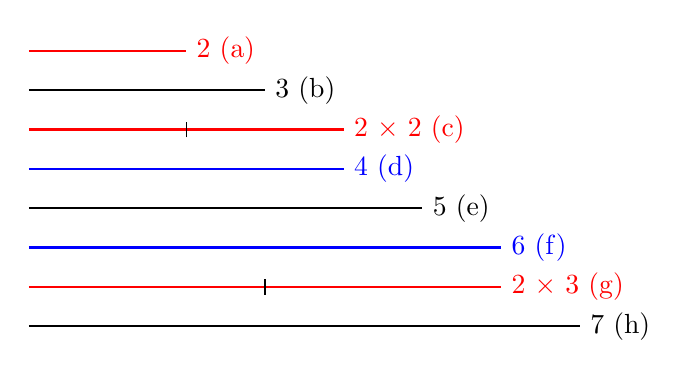
\begin{tikzpicture} 
\draw[red,thick] (0,0) -- (2,0) node[anchor=west]{2 (a)};
\draw[black,thick] (0,-0.5) -- (3,-0.5) node[anchor=west]{3 (b)};
\draw[red, thick] (0,-1) -- (4, -1) node[anchor=west]{2 $\times$ 2 (c)};
\draw[black,thin] (2,-1.1) -- (2,-0.9){}; %line
\draw[blue, thick](0,-1.5) -- (4,-1.5) node[anchor=west]{4 (d)};
\draw[black, thick] (0,-2) -- (5, -2) node[anchor=west]{5 (e)};
\draw[blue, thick] (0,-2.5) -- (6, -2.5) node[anchor=west]{6 (f)};
\draw[red, thick] (0,-3) -- (6, -3) node[anchor=west]{2 $\times$ 3 (g)};
\draw[black,thin] (3,-3.1) -- (3,-2.9){};
\draw[black, thick](0,-3.5) -- (7,-3.5) node[anchor=west]{7 (h)};
\end{tikzpicture}
\caption{A pre-algebraic representation of primes through strings of increasing length}
\label{gr:WhatArePrimes}
\end{figure}

Figure \ref{gr:WhatArePrimes} shows the attempts, through trial and error, to establish which numbers have whole (``integral'') factors and which don't, and while it may be incredibly verbose, it is worth discussing step-by-step. Line $a$ is the first, and can only be divided by 1 (``unity''), and is therefore, \textbf{prime}. Line $b$ cannot be divided into whole multiples of line $a$, therefore $b$ is also prime. line $d$ can be divided into two times line $a$, (as shown with line $c$), therefore $d$ is \textbf{composite}, and so on. Now if we want to establish which numbers are prime from 1 to 10, we will have to do trial divisions for every single number (or line) by every other prime predecessor: a) is 5 divisible by 2? No; b) Is 5 divisible by 3? No \textendash\ then 5 must be prime, and so on with 6, 7, etc.

This allows us to introduce the concept of prime counting function, $\pi(n)$, and through trial divisions up to 10, affirm that $\pi(10)=4$.

\begin{Def}\label{def:Pi(n)}
	Denoted by $\pi(n)$, the prime counting function tells us the exact number of prime numbers less than or equal to some number $n$, or in other words, the \textbf{distribution of primes} less than or equal to $n$.
\end{Def}

Although trial and error seems to include many redundancies, many prime finding algorithms boil down to it. A great example is The Great Internet Mersenne Prime Search \textendash\ GIMPS, a distributed computing effort to find Mersenne primes (see Definition \ref{def:MersennePrimes}). The process consists of, among others, a series of optimised trial divisions and the creation of a modified sieve of Eratosthenes, which will be discussed in detail further in the paper.

\begin{Def} \label{def:MersennePrimes}
	Mersenne primes, denoted by $M_p$, are numbers with form $2^p-1$, such that $M_p$ and $p$ are prime. For example, $M_3 = 2^3-1 = 7$ or $M_5 = 31$.
\end{Def}

The optimised trial divisions are possible due to a few properties of Mersenne primes \textendash\ whose proofs go beyond the scope of this paper \textendash\ which allow to reduce the number of operations that must be performed. Amongst others\citep{GimpsMath}:
\begin{Def}\label{def:PropertiesOfMersennePrimes}
\begin{enumerate}
	\item any factor $q$ of $M_p = 2^p-1$ must have form $2kp+1$. That is, $\frac{M_p}{q} = \frac{2^p-1}{2kp+1} = N, \ N \in \mathbb{N}$.
	\item $q = 1 (\mod 8) \text{ or } 7 (\mod 8)$.
	\item $q$ must be prime.
\end{enumerate}	
\end{Def}

We must also introduce an important definition regarding the magnitude of factor $q$ that will be used throughout this study. If we consider a natural number $n$ such that $q_1 \cdot q_2 = n$, the largest both factors can simultaneously be is $q_1 = q_2 = q$, that is $q^2 = n$, leading to the following definition:
\begin{Def}\label{def:SqrtN}
	The smallest factor of $n$ must be equal to or less than $\sqrt n$.
\end{Def}

To exemplify the process, the primality of two possible Mersenne primes will be checked, $M_{11} = 2^{11}-1 = 2047$  and $M_{17} = 2^{17} - 1 = 131071$. If we first consider $M_{11}$, as per Definition \ref{def:SqrtN}, $q \le \sqrt{2047} \cong 45$, so the first step is to check factor $q = 2kp+1$, replacing k for 1, 2, 3, etc. such that $q \le 45$.
\begin{equation*}
\begin{split}
&\text{For k = 1, } q = 2 \cdot 11 \cdot 1 + 1 = 23 \\
&\text{For k = 2, } q = 45 \\
\end{split}
\end{equation*}
Followed by trial divisions of $M_{11}$ by $q$ such that the result is a natural number (as per Definition \ref{def:PropertiesOfMersennePrimes}.1).
\begin{equation*}
	\frac{2047}{23} = 89
\end{equation*}
Therefore $M_{11}$ is not prime, and we have found its factors: $M_{11} = 23 \cdot 89 = 2047$.
Repeating the process for $M_{17}$, and given that for $M_{17}$, $q \le \sqrt{131071} \cong 362$
\begin{equation*}
\begin{split}
&\text{For k = 1, } q = 2 \cdot 17 \cdot 1 + 1 = 35 \\
&\text{For k = 2, } q = 69 \\
&\text{For k = 3, } q = 103 \\
&q = 137, 171, 205, 239, 273, 307\text{ or }341
\end{split}
\end{equation*}

\vspace{2cm} %formatting
Definition \ref{def:PropertiesOfMersennePrimes}.2 tells us that q = 1 or 7 (mod 8):
\begin{table} [h]
	\centering
\begin{tabular} {c c c}
\sout{$35 \mod 8 = 3$}		& \sout{$171 \mod 8 = 3$}	& $273 \mod 8 = 1 $ \\
\sout{$69 \mod 8 = 5$}		& \sout{$205 \mod 8 = 5$}	& \sout{$ 307 \mod 8 = 3 $}\\
$103 \mod 8 = 7$	& $239 \mod 8 = 7$	& \sout{$ 341 \mod 8 = 5 $}\\
$137 \mod 8 = 1$ 
\end{tabular}
\end{table}

Finally, as per Definition \ref{def:PropertiesOfMersennePrimes}.3 and indeed Theorem \ref{thm:FTA}, 273 is excluded for being composite ($3\cdot7\cdot13 = 273$). Therefore only the following trial divisions must be performed in order to verify the primality of 131071:
\begin{equation*}
\begin{split}
	\frac{131071}{103} = 1272 + \frac{55}{103}  \quad\text{or }\quad \frac{131071}{137} = 956 + \frac{99}{137} \\[2ex]
	\text{or} \quad \frac{131071}{239} = 548 + \frac{99}{239} \quad\text{or }\quad \frac{131071}{273} = 480 + \frac{31}{273} \\[2ex]
\end{split}
\end{equation*}

None of which resulted in natural numbers, and thus $M_{17} = 131071$ is prime. This means that with four trial divisions, we were able to with certainty establish that $131071$ is prime! Indeed, these optimisations are so powerful that the current largest prime has over 22 million digits and was found through GIMPS utilising, amongst others, this method. Figure \ref{gr:MersennePrimes} gives a great insight into the incredible jump in size of primes found in the last circa 20 years since its inception \textendash\ from around 420,000 digits in 1996 to 10,00,000 in 2006 to 22,000,000 in 2016.

It is clear that this efficiency is only applicable to a very narrow scope, and serves the purpose of checking the primality of a fairly specific set of numbers. There is, in fact, a method that contrasts greatly to performing trial divisions for each number, and it is called a sieve of Erastothenes. 

\begin{figure} [h]
	\caption{Distribution of GIMPS-found Mersenne primes \citep{GimpsFoundNumbers}.}
	\label{gr:MersennePrimes}
	\begin{tikzpicture}
	\begin{axis}[
	scaled y ticks = false,
	xlabel={Year},
	ymajorgrids,
	xticklabel style={/pgf/number format/1000 sep=, anchor=north, font=\scriptsize},
	xmin=1995, xmax=2017,
	ylabel={Number length},
	]
	\addplot[color=blue, mark=square, only marks]
	table {MersennePrimes.dat};
	\end{axis}
	\end{tikzpicture}
\end{figure}
\vspace{5cm} %formatting